% !TeX encoding = UTF-8
% !TeX spellcheck = en_US
% !TeX root = presentation.tex
\subsection{KUKA youBot}
\begin{frame}{youBot Driver}

\begin{itemize}
	\item \textbf{ROS Wrapper}
	\begin{itemize}
		\item Allows to write ROS programs for controlling youBot
		\item Provides an interface between youBot driver and ROS framework
		\item Allows to move the base and arm by sending ROS messages
	\end{itemize}
	\item \textbf{List of Drivers}
		\begin{itemize}
			\item Drive base
			\item Laser scanners
			\item Arm 
			\item Joystick
			\item Transformations
		\end{itemize}
\end{itemize}
  
\end{frame}


\begin{frame}{Map building II}
\begin{itemize}
	\item \textbf{Problems}
		\begin{itemize}
			\item Messy Map
		\end{itemize}
	\item \textbf{Solutions}
		\begin{itemize}
			\item Incorrect transformation between laser frame and base link
		\end{itemize}
\end{itemize}
\end{frame}
\begin{frame}{Map building III}
    \centering
    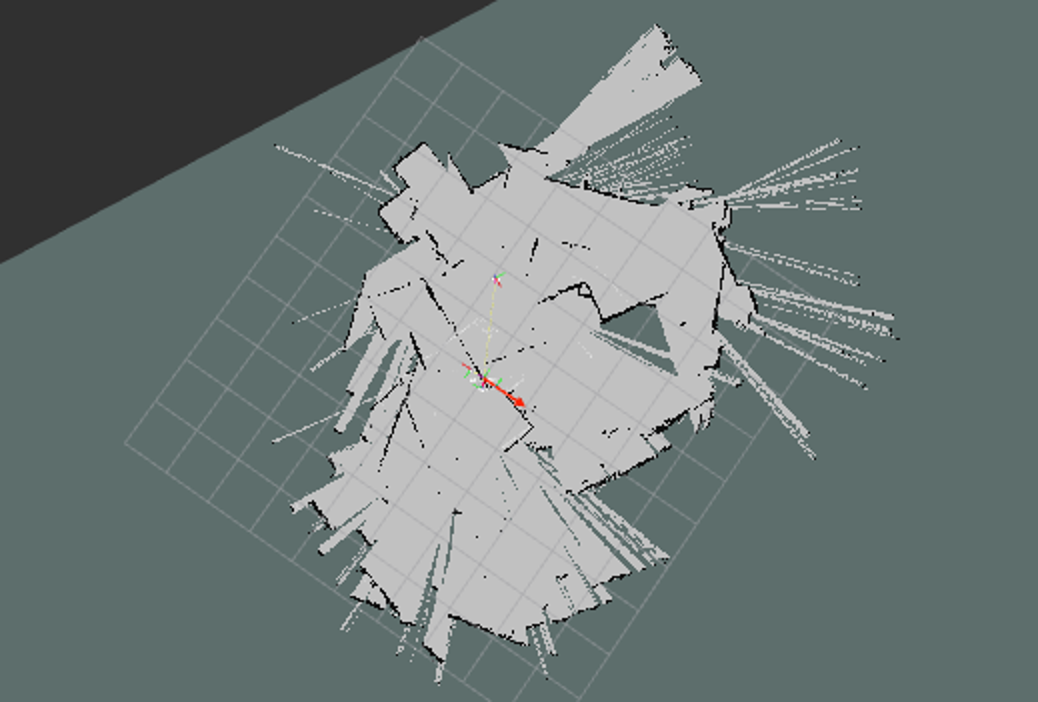
\includegraphics[width=0.9\textwidth]{gfx/map_messy.png}
\end{frame}
\begin{frame}{Map building IV}
\centering
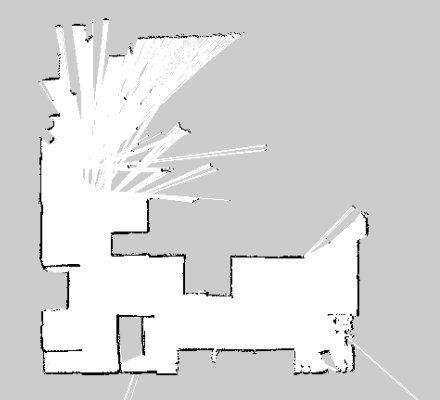
\includegraphics[width=0.8\textwidth]{gfx/map.png}
\end{frame}
\begin{frame}{Localization II}
\end{frame}
\begin{frame}{Navigation}
\end{frame}
\begin{frame}{Navigation - Local Planner}
\end{frame}
\begin{frame}{BNT.py}
    
    The node acts as path executor that reads  a set of user inputs and convert them to move\_base\_msgs.
    \begin{itemize}
        \item Class: Position, Pose, Environment, Workspace, PathExecutor
        
        \item Functions:
        \begin{itemize}
            \item 
            \item Clear cost map
            \item 
        \end{itemize}
    \end{itemize}
    
\end{frame}
